\chapter{Clustering: Finding Out the Districts with High and Low Risks of Floods}

By now, the correlation between rainfall rate and flood occurrences is already known. Moreover, the amount of sub-districts and people that will be affected by floods in any given rainfall rate can be predicted with linear regression model and third order polynomial regression model. Next, the problem is: the authorities now can predict the amount of sub-districts that will be flooded when the heavy rainfall pours down the city, but where should they focus their attention to? is there any particular district that they should take their attention to?\\

\noindent
In order to answer this question, in this chapter, all of the districts in Jakarta will be clustered into certain number of segments. From that, the classification regarding their potential risks of upcoming floods can be concluded.\\

\section{Feature Extractions}
Before clustering all of the districts in Jakarta into several segments, the first that needs to be done is to obtain the list containing the name of all of the districts. This is necessary because the investigation will be conducted at the district level instead of sub-district level to avoid the visualization that is too dense. Afterall, each district also represents several sub-districts. This means that all of the features in each sub-district will be assigned and aggregated to the district in which they are located.\\

\noindent
In order to obtain all of the districts name, web-scraping technique from five different Wikipedia pages is applied. This task can be done with relevant libraries in Python such as pandas and BeautifulSoup to parse the HTML and convert it to a data frame.\\

\noindent
After the extraction of the names of all of the districts in Jakarta, the next step is to obtain the latitude and longitude coordinates of each district. This task can be completed by utilizing geopy library in Python. After all of the necessary information is obtained, then the geospatial visualization of the districts in Jakarta can be shown using folium library. The visualization is shown in Figure \ref{fig=map.png}.\\

\begin{figure}
\begin{center}
\graphicspath{ {./Pict/} }
\includegraphics[scale=0.8]{map.png}
\caption{Geospatial visualization of the districts of Jakarta}\label{fig=map.png}
\end{center}
\end{figure}


\noindent
After visualization, then the features that are relevant for clustering need to be extracted. With meaningful features, then the clustering algorithm such as k-Means would perform better and will give a precise clustering result. In order to obtain meaningful features to help the clustering algorithm to make a clustering decision, more than 30 datasets from Satu Data Indonesia website will be fetched and combined into one data frame.\\

\noindent
Each of the dataset from Satu Data Indonesia contains flood occurrences in Jakarta within a month. The data that are available are the one in the span 2013 until 2016, which means that in total there should be 48 different datasets. However, there were few months where the datasets are unavailable. The missing dataset in certain months wouldn't matter much since for this chapter, the focus is not about predicting the trend, but to segmenting the districts. In order to segment the districts, the most important thing is the aggregation of all of the features to provide meaningful clustering results.\\

\noindent
In the end, the features that are extracted and converted into the final data frame are:
\begin{itemize}
\item The number of cases of floods in each sub-district.
\item The number of people who are affected by floods.
\item The number of people who are forced to relocate from their own house.
\item The number of days needed for each district to recover from each flood occurrence.
\end{itemize}

\section{Determining the Number of Cluster}
For the clustering of the districts in Jakarta, an unsupervised machine learning algorithm, which is k-Means clustering, will be applied. However, before the clustering is conducted, one important thing that should be done in advance is to choose the number of clusters. It is tricky to know the optimum number of cluster in advance without doing a simulation. Applying too little number of cluster would yield to a very high cost function while applying too many number of cluster will yield to meaningless result.\\

\begin{figure}
\begin{center}
\graphicspath{ {./Pict/} }
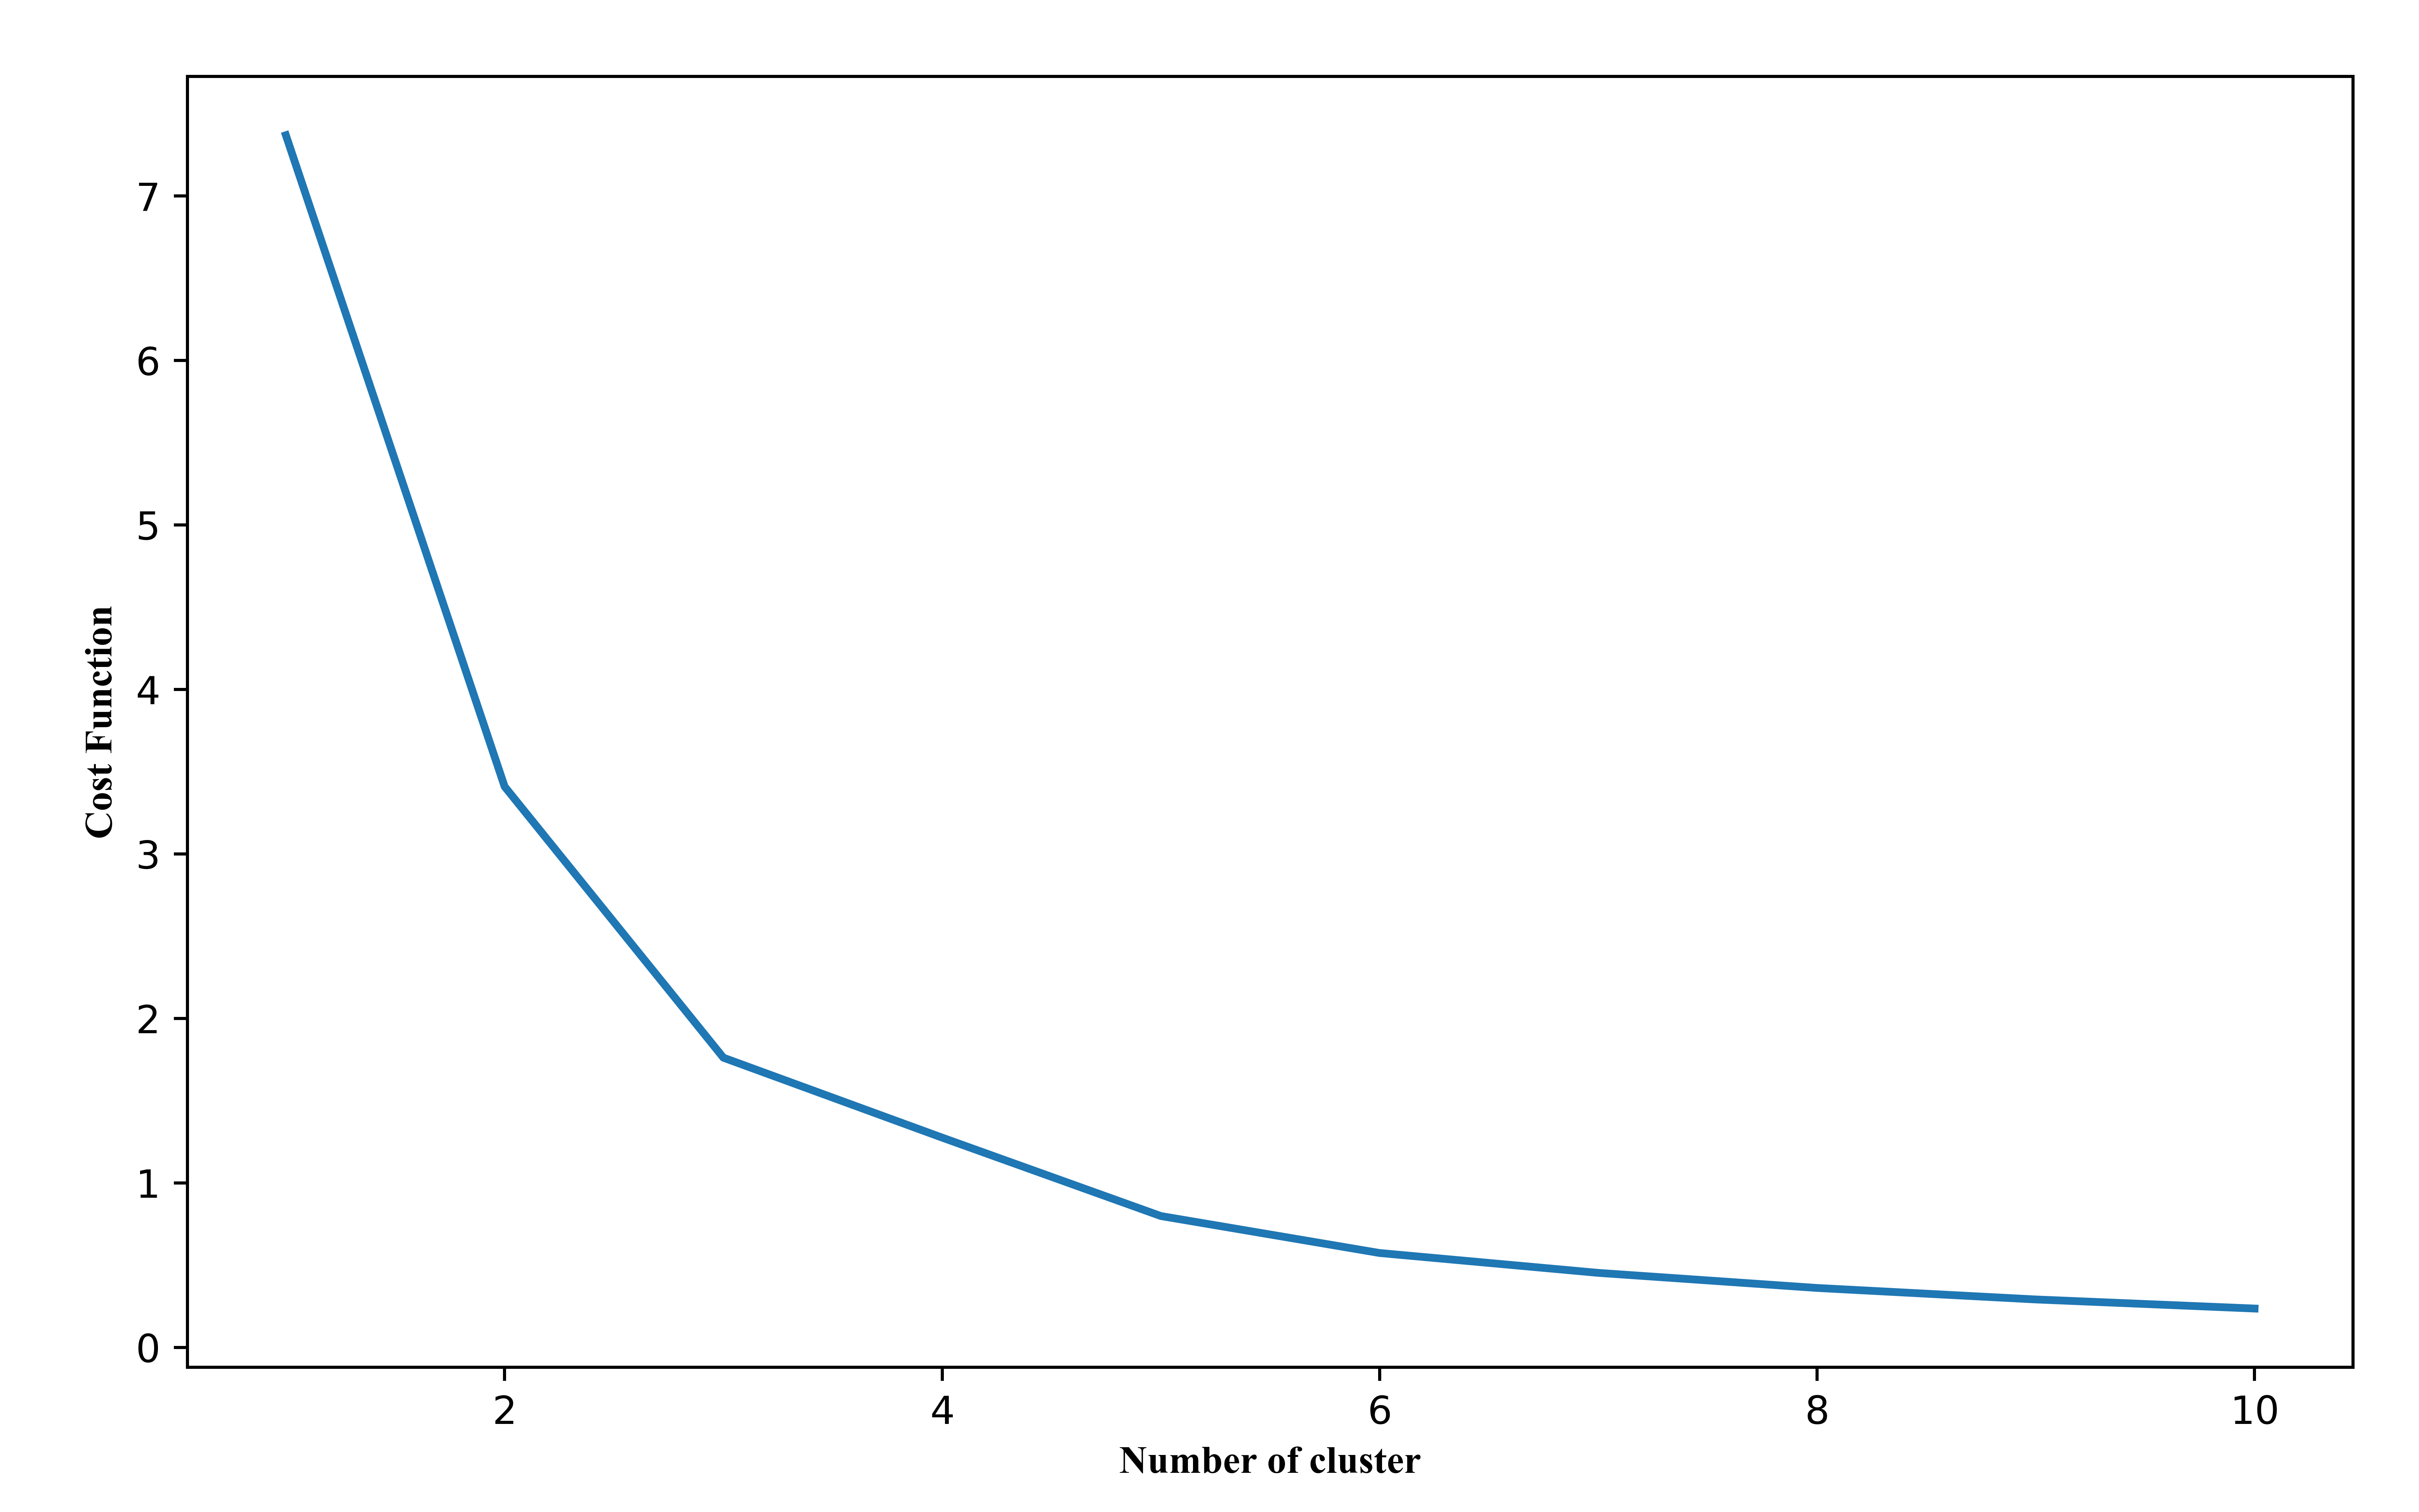
\includegraphics[scale=0.15]{kcluster.png}
\caption{Elbow method to determine optimum number of cluster. Optimum number of cluster= 3}\label{fig=kcluster.png}
\end{center}
\end{figure}

\noindent
In order to know the optimum number of cluster, the elbow method is going to be applied. The elbow method is a very helpful method to get the number of clusters that gives less cost function but at the same time still retains the meaningfulness of the result. Figure \ref{fig=kcluster.png} shows the simulation result of the elbow method. It is clear from the graph that the optimum number of cluster would be 3.

\section{Clustering}
Knowing that 3 clusters will give the optimum result, then the K-Means clustering algorithm can be applied. Figure \ref{fig=cluster.png} shows the clustering result in a map. \\

\begin{figure}
\begin{center}
\graphicspath{ {./Pict/} }
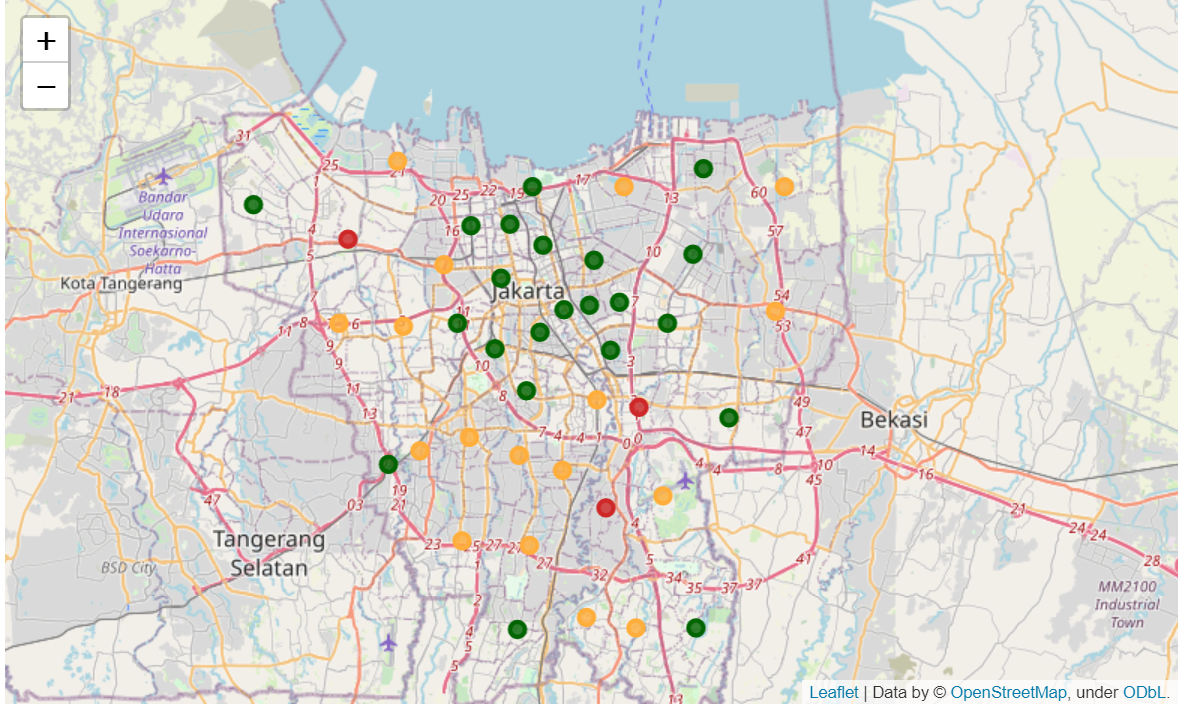
\includegraphics[scale=0.8]{cluster.png}
\caption{Clustering result of the districts of Jakarta. Green: Safe, Orange: Moderate, Red: High Risks of Flooding}\label{fig=cluster.png}
\end{center}
\end{figure}

\noindent
In order to understand better the characteristics of each cluster, Table \ref{tab:1}, Table \ref{tab:2}, and Table \ref{tab:3} give the overview regarding the result for each cluster.\\
\begin{table}
\centering
\caption{Cluster 1: The safest districts in Jakarta}
\label{tab:1}
\begin{adjustbox}{width=\textwidth}
\begin{tabular}{llrrrrrrr}
\toprule
{} &       District &  Latitude &   Longitude &  Cluster Labels &  no. of cases &  no. of People Affected &  no. of People Forced to Relocate &  Days of Flood Recovery \\
\midrule
0  &           Koja & -6.120750 &  106.907362 &               1 &            16 &                  4236.0 &                              6067 &                    52.0 \\
5  &     Pademangan & -6.129052 &  106.828972 &               1 &            12 &                  1935.0 &                              1453 &                    37.0 \\
6  &       Cipayung & -6.329399 &  106.903739 &               1 &            14 &                  1225.0 &                               801 &                    50.0 \\
7  &    Duren Sawit & -6.234138 &  106.919247 &               1 &            10 &                   648.0 &                               150 &                    25.0 \\
8  &      Kalideres & -6.137006 &  106.701594 &               1 &            16 &                 24392.0 &                             14180 &                    66.0 \\
11 &       Palmerah & -6.191002 &  106.794363 &               1 &            10 &                 27987.0 &                             20253 &                    32.0 \\
13 &      Kemayoran & -6.162546 &  106.856890 &               1 &             8 &                   300.0 &                               300 &                    47.0 \\
15 &          Senen & -6.184971 &  106.843235 &               1 &             0 &                     0.0 &                                 0 &                     0.0 \\
18 &     Taman Sari & -6.146142 &  106.818499 &               1 &             6 &                     0.0 &                               659 &                    19.0 \\
21 &       Matraman & -6.203624 &  106.864579 &               1 &             9 &                  2844.0 &                              2259 &                    21.0 \\
22 &         Gambir & -6.170300 &  106.814800 &               1 &             3 &                     0.0 &                                 0 &                     7.0 \\
23 &        Menteng & -6.195026 &  106.832224 &               1 &             2 &                     0.0 &                                 0 &                     6.0 \\
24 &    Pulo Gadung & -6.191109 &  106.890605 &               1 &             0 &                     0.0 &                                 0 &                     0.0 \\
25 &     Johar Baru & -6.183125 &  106.855332 &               1 &             4 &                     0.0 &                                 0 &                    11.0 \\
26 &  Kelapa Gading & -6.159938 &  106.902483 &               1 &            13 &                  6537.0 &                              8667 &                    48.0 \\
28 &      Setiabudi & -6.221706 &  106.826308 &               1 &             4 &                    30.0 &                               690 &                     6.0 \\
30 &        Tambora & -6.146614 &  106.801046 &               1 &            16 &                   523.0 &                             12772 &                    81.0 \\
32 &      Jagakarsa & -6.330101 &  106.822237 &               1 &            17 &                  2736.0 &                              1737 &                    51.0 \\
35 &    Sawah Besar & -6.155891 &  106.833580 &               1 &             9 &                 17376.0 &                               110 &                    17.0 \\
37 &  Cempaka Putih & -6.181214 &  106.868548 &               1 &             1 &                     0.0 &                                 0 &                     2.0 \\
39 &   Pesanggrahan & -6.255458 &  106.763112 &               1 &            22 &                  7589.0 &                              1020 &                    62.0 \\
40 &    Tanah Abang & -6.202400 &  106.811900 &               1 &            14 &                 51860.0 &                             10002 &                    60.0 \\
\bottomrule
\end{tabular}
\end{adjustbox}
\end{table}

\begin{table}
\centering
\caption{Cluster 2: The districts with highest risks of flooding in Jakarta}
\label{tab:2}
\begin{adjustbox}{width=\textwidth}
\begin{tabular}{llrrrrrrr}
\toprule
{} &     District &  Latitude &   Longitude &  Cluster Labels &  no. of cases &  no. of People Affected &  no. of People Forced to Relocate &  Days of Flood Recovery \\
\midrule
12 &  Kramat Jati & -6.274940 &  106.862501 &               2 &            74 &                170580.0 &                             35631 &                   256.0 \\
33 &   Cengkareng & -6.152899 &  106.744718 &               2 &            51 &                828568.0 &                             81643 &                   231.0 \\
36 &   Jatinegara & -6.229147 &  106.877417 &               2 &            64 &                421638.0 &                             52174 &                   312.0 \\
\bottomrule
\end{tabular}
\end{adjustbox}
\end{table}

\begin{table}
\centering
\caption{Cluster 3: The districts with moderate risks of flooding in Jakarta}
\label{tab:3}
\begin{adjustbox}{width=\textwidth}
\begin{tabular}{llrrrrrrr}
\toprule
{} &           District &  Latitude &   Longitude &  Cluster Labels &  no. of cases &  no. of People Affected &  no. of People Forced to Relocate &  Days of Flood Recovery \\
\midrule
1  &           Cilandak & -6.289798 &  106.796926 &               3 &            35 &                 28333.0 &                               913 &                    89.0 \\
2  &          Kembangan & -6.191395 &  106.740586 &               3 &            28 &                 60905.0 &                              1074 &                    72.0 \\
3  &      Tanjung Priok & -6.128858 &  106.870793 &               3 &            28 &                 91260.0 &                             35521 &                    97.0 \\
4  &        Kebon Jeruk & -6.192572 &  106.769725 &               3 &            43 &                177859.0 &                             14695 &                   139.0 \\
9  &             Cakung & -6.185562 &  106.940109 &               3 &            22 &                 25121.0 &                              5614 &                   106.0 \\
10 &            Makasar & -6.269587 &  106.888697 &               3 &            38 &                 33301.0 &                              5101 &                   120.0 \\
14 &        Penjaringan & -6.117265 &  106.767433 &               3 &            28 &                 42330.0 &                             43968 &                   142.0 \\
16 &     Kebayoran Baru & -6.243164 &  106.799850 &               3 &            29 &                 34747.0 &                               524 &                    80.0 \\
17 &       Pasar Minggu & -6.291950 &  106.827835 &               3 &            32 &                 31648.0 &                              7946 &                    93.0 \\
19 &            Ciracas & -6.329635 &  106.876604 &               3 &            26 &                 12941.0 &                               984 &                    60.0 \\
20 &           Pancoran & -6.258085 &  106.842733 &               3 &            43 &                 36566.0 &                             14158 &                   156.0 \\
27 &     Kebayoran Lama & -6.249128 &  106.777782 &               3 &            40 &                 10833.0 &                               801 &                   107.0 \\
29 &              Tebet & -6.226016 &  106.858396 &               3 &            41 &                140138.0 &                             31043 &                   177.0 \\
31 &         Pasar Rebo & -6.324973 &  106.853376 &               3 &            26 &                  4957.0 &                                18 &                    81.0 \\
34 &          Cilincing & -6.129015 &  106.944454 &               3 &            33 &                 45478.0 &                             23646 &                   118.0 \\
38 &  Grogol Petamburan & -6.164188 &  106.788317 &               3 &            31 &                  5746.0 &                              7590 &                   120.0 \\
41 &   Mampang Prapatan & -6.250878 &  106.823021 &               3 &            36 &                  6995.0 &                              2246 &                    81.0 \\
\bottomrule
\end{tabular}
\end{adjustbox}
\end{table}

\noindent
From Table \ref{tab:1} it can be seen that the districts that contained in cluster 1 are the safest districts in Jakarta in terms of their robustness against flooding, although they are not entirely safe. In general, the districts that clustered together in this cluster have the lowest number of flood cases over the span 2013 until 2016 and they also only need short amount of time to recover from floods.\\

\noindent
There are only three districts in cluster 2, as shown in Table \ref{tab:2}. However, these three are the districts with the highest potential to have upcoming floods should a heavy rainfall pours down Jakarta in the future. As shown in the table, these three districts have by far the most cases of floods over the span 2013 until 2016, the most people who are affected by floods, and they also take the longest time to recover from floods. Without a doubt, these three districts are the one that the authorities, the rescue team, and the medical teams should focus their attention the most to.\\

\noindent
In cluster 3, as shown in Table \ref{tab:3}, there are several districts that have lower number in terms of people affected by flood compared to some districts in cluster 1. However, by taking a closer look, all of the districts in cluster 3 have more number of flood cases and they need longer time to recover from floods compared to cluster 1. At the same time, they are also not as severe as the three districts in cluster 2. In conclusion, the districts in cluster 3 are the districts that need moderate amount of attention should a heavy rainfall pours down Jakarta.\\


